\begin{figure}[htbp]
\centering
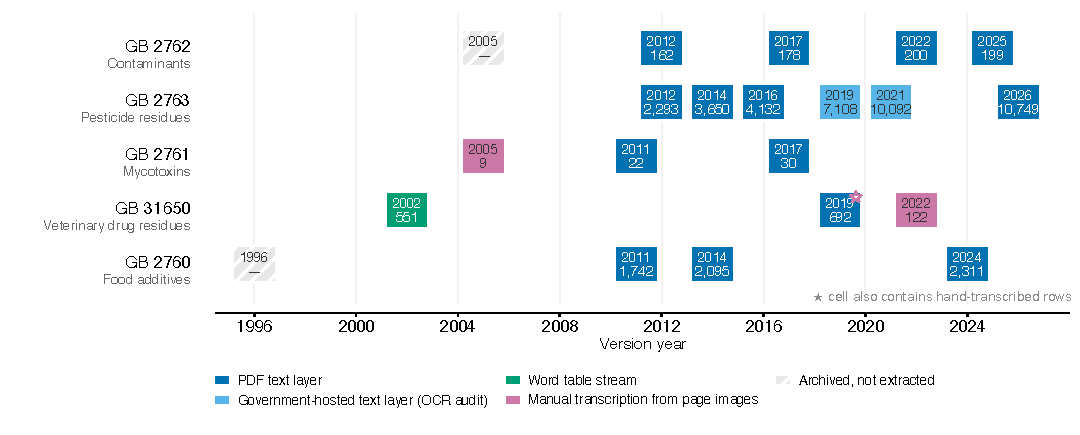
\includegraphics[width=\textwidth]{Results/fig/fig1Coverage.pdf}
\caption{Coverage matrix. Rows are the five standard families and columns are version years from 1996 to 2026. Each cell gives the number of released limit records and is shaded by read path. The 2019 and 2021 pesticide cells use government-hosted copies. The edition scans, kept as audit-only copies, anchor edition identity and supply a frozen optical-character-recognition (OCR) cross-check. A star marks a mainly machine-read cell with hand-transcribed rows. The two hatched cells, GB 2762-2005 and GB 2760-1996, are archived but unextracted. The matrix holds 21 coverage cells, and the 19 extracted cells contain 46,337 records. The 2002 veterinary-drug cell is Ministry of Agriculture Announcement 235, and its 2022 cell is the supplementary standard GB 31650.1.}
\label{fig1Coverage}
\end{figure}
